\documentclass[11pt,fleqn]{article}
\usepackage{graphicx}
\usepackage[letterpaper, margin=1in]{geometry}
\usepackage{hyperref}
\usepackage{multicol}
\usepackage[toc,page]{appendix}
\usepackage{amsmath}

\hypersetup{colorlinks=true, linktoc=all, linkcolor=blue}

\begin{document}

\begin{center}
\Large{\textbf{Stereo Vision Report}}\\[5pt]
\large{Robert Washbourne}\\
Last edited: \today
\end{center}

\tableofcontents

% .......................................................................................................
\section{Introduction}
% .......................................................................................................

Imagine driving in the dark, alert but not noticing a deer cross the road. Using stereo matching methods to see what is close, your car could detect the deer and brake before you even saw the obstacle. The cameras would find distances, and sensing something closer than 20 feet, send the location of the deer to the computer. The computer would see that driving over this would be catastrophic for the car, and turn on the brakes. The deer, and you, would be safe.


% .......................................................................................................
\section{What is Stereo Matching}
% .......................................................................................................

Stereo matching is a topic in computer vision where two images, taken from aligned cameras several centimetres apart, are processed and depth data is returned. For example, taking two images and using a simple algorithm, a grayscale image is returned, with lighter pixels closer then darker pixels.\\[6pt]
%
See figure \ref{fig:example1} for an example.

%\begin{tabular}{ccc}\\
%\hline
%\texttt{Left} & \texttt{Right} & \texttt{Disparity} \\
%\end{tabular}

%\newpage
%\begin{figure}[!ht]
%\centering
%a) 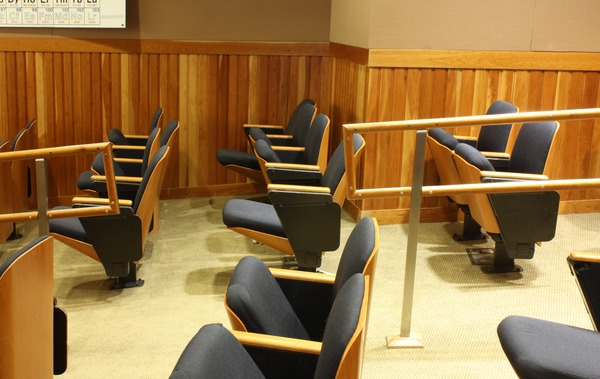
\includegraphics[width=0.6\textwidth]{images/im0-600.jpg} \\[10pt]
%b) 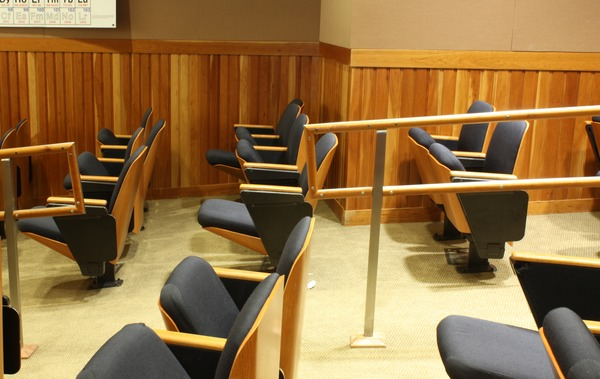
\includegraphics[width=0.6\textwidth]{images/im1-600.jpg} \\[10pt]
%c) 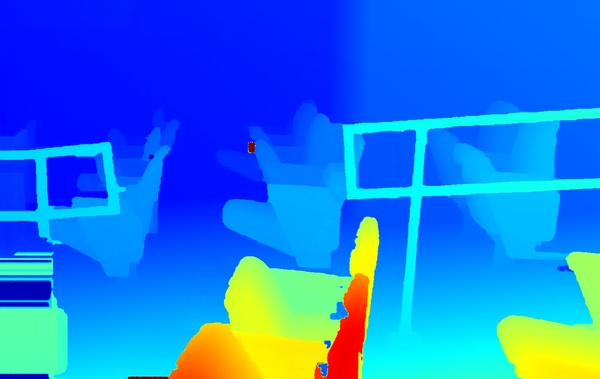
\includegraphics[width=0.6\textwidth]{images/disp-600.jpg} \\[10pt]
%\label{fig:example1}
%\caption{Example of disparity matching. a) image from left camera b) image from right camera c) disparity map}
%\end{figure}

\begin{figure}[!ht]
\label{fig:example1}
\centering
\setlength\tabcolsep{0.005\textwidth}
\begin{tabular}{ccc}
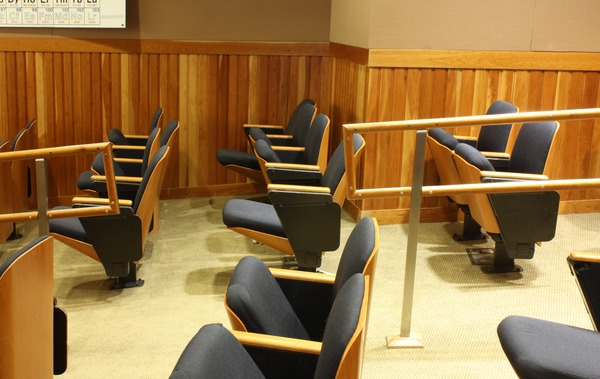
\includegraphics[width=0.33\textwidth]{images/im0-600.jpg} &
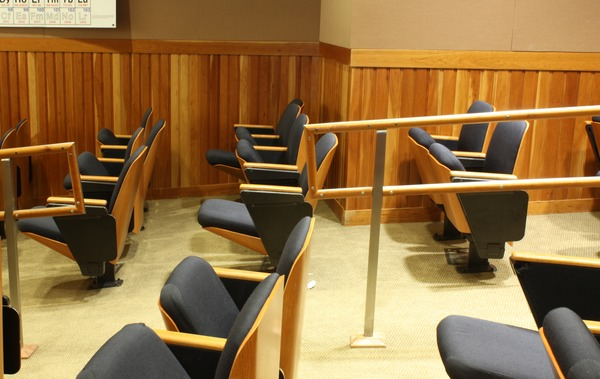
\includegraphics[width=0.33\textwidth]{images/im1-600.jpg} &
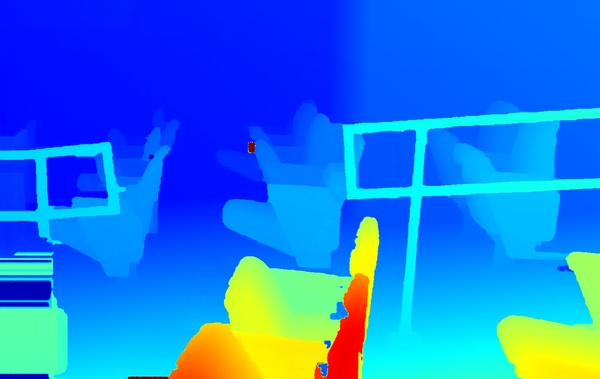
\includegraphics[width=0.33\textwidth]{images/disp-600.jpg} \\[2pt]
a) & b) & c) \\
\end{tabular}
\caption{Example of disparity matching. a) Image from left camera. b) Image from right camera c) Disparity map.}
\end{figure}


% .......................................................................................................
\section{Methods}
% .......................................................................................................
There are several methods of creating depth maps.
They can be created by a laser scanner, but this process is much slower than stereo matching, and unsuited for real time processing. They can also be created with two cameras. This is the method that I explored, as it is fast enough for realtime processing, and yields good results. In this image, a colormap is used to make it easier to see what is closer. The blues are at the back and the reds at at the front.

\subsection{Result Comparison}
\begin{figure}[!ht]
\label{fig:result1}
\centering
\setlength\tabcolsep{0.005\textwidth}
\begin{tabular}{ccc}
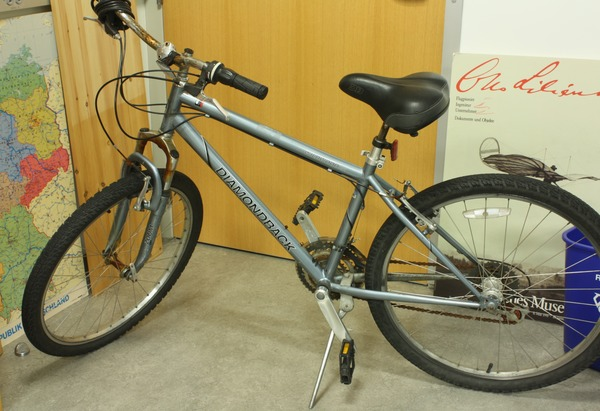
\includegraphics[width=0.33\textwidth]{images/_im0-600.jpg} &
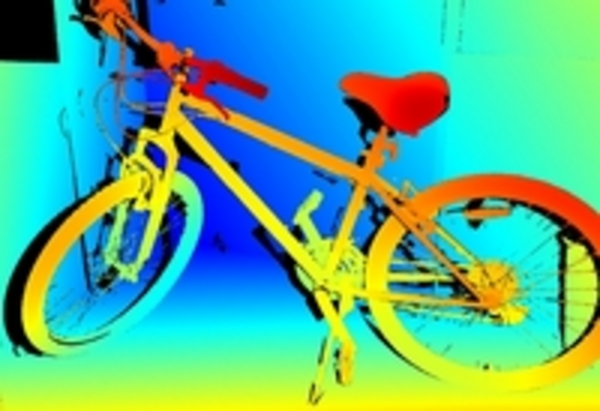
\includegraphics[width=0.33\textwidth]{images/disp0GT-600.jpg} &
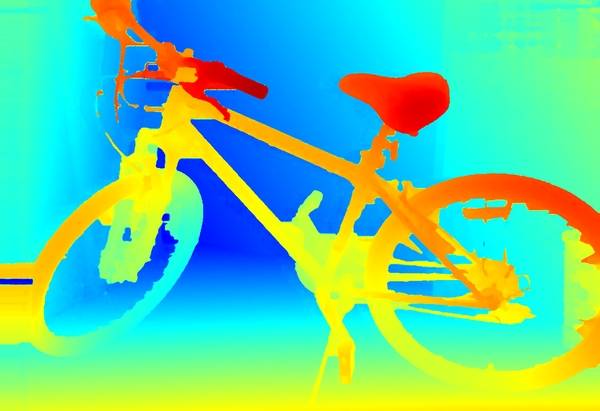
\includegraphics[width=0.33\textwidth]{images/_disp-600.jpg} \\[2pt]
a) & b) & c) \\
\end{tabular}
\caption{Comparison of laser and stereo. a) Original image b) Laser result c) Stereo matching result.}
\end{figure}

The laser result is crisper, but it takes much longer to generate. The stereo matching result is worse, with parts of the image blended, but it was generated much faster. 


% .......................................................................................................
\section{Workflow}
% .......................................................................................................

\subsection{Capture images from both webcams}  

\subsection{Split images into 1 pixel high rows}

This picture is a comparison of a row of the left image and the row of the right image. \\
The data is shifted by around 60 pixels everywhere on the line.

\begin{figure}[!ht]
\label{fig:strips}
\centering
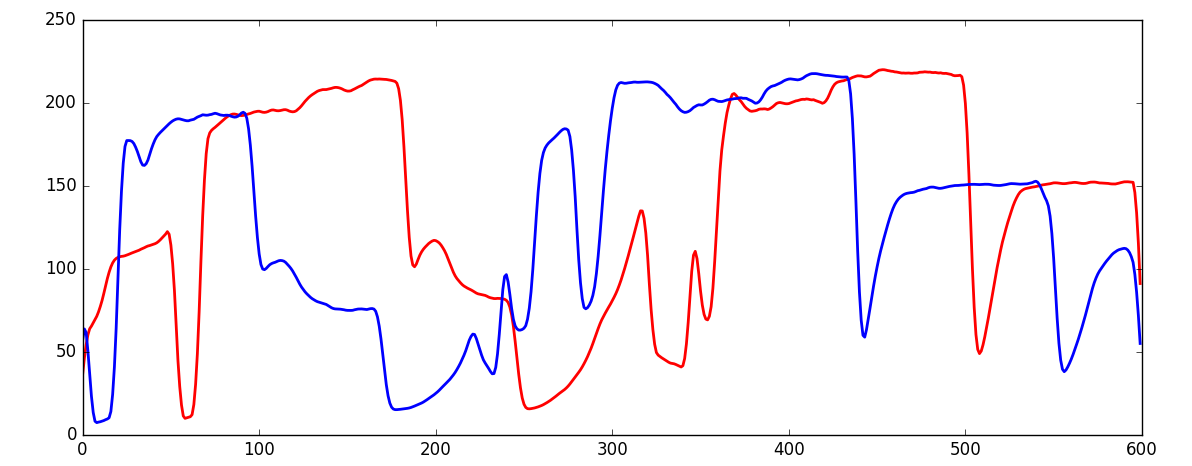
\includegraphics[width=1\textwidth]{images/strips.png} \\[2pt]
\caption{1 pixel strips from the images shown in Figure \ref{fig:example1}. Left image blue line, and right image red line. Left axis is the pixels value of the point of the bottom axis. For example, at 300, the blue line is around 200.}
\end{figure}

\subsection{Correlate image strips from left and right images}
For each pixel in the row of the left image, a window is slid along the right image's row to find a match for that pixel.\\
If we did it for the 100th pixel of the blue line in the rows in figure 2, we would find that the corresponding red point is 80 pixels to the right.

\subsection{Estimate pixel distance}
The pixel distance that we found is added to the relevant row of the disparity matrix.

\subsection{Apply edge preserving filter to remove noise}
Using a median filter, a lot of noise can be removed. A median filter is a square window that moves around every pixel, and changes the pixel to the median of the pixels inside the square.\\
Say that you have a 3 by 3 median filter, and it passes over this part of the image (Because this is a 4 x 4 matrix, the operation will only be conducted for the inner pixels):

\[ \left( \begin{array}{cccc}
2 & 0 & 3 & 5 \\
1 & 4 & 2 & 7 \\
3 & 1 & 0 & 3 \\
6 & 8 & 4 & 2 \\ 
\end{array} \right)
\rightarrow
\left(\begin{array}{ccc}
2 & 0 & 3 \\
1 & 4 & 2 \\
3 & 1 & 0 \\
\end{array} \right)
\left(\begin{array}{ccc}
0 & 3 & 5 \\
4 & 2 & 7 \\
1 & 0 & 3 \\
\end{array} \right)
\left(\begin{array}{ccc}
4 & 2 & 7 \\
1 & 0 & 3 \\
8 & 4 & 2 \\
\end{array} \right)
\left(\begin{array}{ccc}
1 & 4 & 2 \\
3 & 1 & 0 \\
6 & 8 & 4 \\
\end{array} \right)\]
We see that the medians of the 3x3 matrixes are
\begin{equation} \label{eq1}
\begin{split}
(0,0,1,1,2,2,3,3,4) = 2\\
(0,0,1,2,3,3,4,5,7) = 3\\
(0,1,2,2,3,4,4,7,8) = 3\\
(0,1,1,2,3,4,4,6,8) = 3\\
\end{split}
\end{equation}


\begin{equation}
\begin{aligned}
\begin{bmatrix}
2 & 0 & 3 & 5 \\
1 & 4 & 2 & 7 \\
3 & 1 & 0 & 3 \\
6 & 8 & 4 & 2 \\ 
\end{bmatrix}
\end{aligned}
\end{equation}


\newpage
\subsubsection{Illustration of median filter}

A median filter works by applying a particular type of edge preserving averaging to pixels. Median filtering is quite simple, only two steps:
\begin{enumerate}
\item sort the samples in the input filter window by magnitude
\item take the median sample value as the output
\end{enumerate}
%
\begin{equation*}
\begin{aligned}
&\texttt{4x4 section of representative input image data}\\
& \hspace{20pt} \begin{bmatrix}
2 & 0 & 3 & 5 \\
1 & 4 & 2 & 7 \\
3 & 1 & 0 & 3 \\
6 & 8 & 4 & 2 \\ 
\end{bmatrix} \\[10pt]
%
& \texttt{Application of 3x3 median filter to the $(2,2)$ interior filter location}\\
& \hspace{20pt} \begin{bmatrix}
\mathbf{2} & \mathbf{0} & \mathbf{3} & 5 \\
\mathbf{1} & \mathbf{4} & \mathbf{2} & 7 \\
\mathbf{3} & \mathbf{1} & \mathbf{0} & 3 \\
6 & 8 & 4 & 2 \\ 
\end{bmatrix} 
\rightarrow (2, 0, 3, 1, 4, 2, 3, 1, 0) \rightarrow (0, 0, 1, 1, 2, 2, 3, 3, 4) \rightarrow (2) \\[10pt]
%
& \texttt{Application of 3x3 median filter to the $(2,3)$ interior filter location}\\
& \hspace{20pt} \begin{bmatrix}
2 & \mathbf{0} & \mathbf{3} & \mathbf{5} \\
1 & \mathbf{4} & \mathbf{2} & \mathbf{7} \\
3 & \mathbf{1} & \mathbf{0} & \mathbf{3} \\
6 & 8 & 4 & 2 \\ 
\end{bmatrix} 
\rightarrow (0, 3, 5, 4, 2, 7, 1, 0, 3) \rightarrow (0, 0, 1, 2, 3, 4, 4, 5, 7) \rightarrow (3) \\[10pt]
%
& \texttt{Application of 3x3 median filter to the $(3,2)$ interior filter location}\\
& \hspace{20pt} \begin{bmatrix}
2 & 0 & 3 & 5 \\
\mathbf{1} & \mathbf{4} & \mathbf{2} & 7 \\
\mathbf{3} & \mathbf{1} & \mathbf{0} & 3 \\
\mathbf{6} & \mathbf{8} & \mathbf{4} & 2 \\ 
\end{bmatrix} 
\rightarrow (1, 4, 2, 3, 1, 0, 6, 8, 4) \rightarrow (0, 1, 1, 2, 3, 4, 4, 6, 8) \rightarrow (3) \\[10pt]
%
& \texttt{Application of 3x3 median filter to the $(3,3)$ interior filter location}\\
& \hspace{20pt} \begin{bmatrix}
2 & 0 & 3 & 5 \\
1 & \mathbf{4} & \mathbf{2} & \mathbf{7} \\
3 & \mathbf{1} & \mathbf{0} & \mathbf{3} \\
6 & \mathbf{8} & \mathbf{4} & \mathbf{2} \\ 
\end{bmatrix} 
\rightarrow (4, 2, 7, 1, 0, 3, 8, 4, 2) \rightarrow (0, 1, 2, 2, 3, 4, 4, 7, 8) \rightarrow (3) \\[10pt]
%
& \texttt{Output 3x3 median filtered data, with edge locations zeroed}\\
& \hspace{20pt} \begin{bmatrix}
0 & 0 & 0 & 0 \\
0 & 2 & 3 & 0 \\
0 & 3 & 3 & 0 \\
0 & 0 & 0 & 0 \\ 
\end{bmatrix} \\[10pt]
\end{aligned}
\end{equation*}

HELLLO
helefef

\subsection{Return the final disparity map}

The disparity map matrix would range in values that did not show distance. To turn these values into distances, the program triangulates using the distance between cameras.

\section{Setup}
My setup is a wooden board with 2 Microsoft LifeCam 3000 webcams 2 centimeters apart, facing the same direction. It can see everything farther than three feet away, and works indoors and outdoors.\\[2pt]

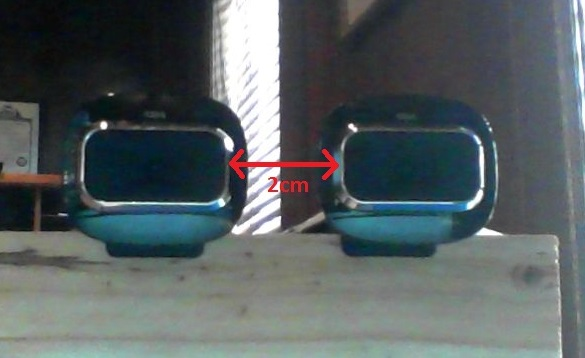
\includegraphics[width=0.95\textwidth]{images/setup.jpg}


\begin{appendices}

% .......................................................................................................
\section{References}
% .......................................................................................................

this needs work

\begin{enumerate}
\item Middlebury Computer Vision dataset
http://vision.middlebury.edu for the example images and laser vs stereo matching comparison. (http://vision.middlebury.edu)
\item http://vision.middlebury.edu/stereo/datasets3/test/Classroom2/im0-600.jpg
\item http://vision.middlebury.edu/stereo/datasets3/test/Classroom2/im1-600.jpg
\item http://vision.middlebury.edu/stereo/results3/outputs/alg0034/test/Classroom2/disp-600.jpg
\end{enumerate}


% .......................................................................................................
\section{Definitions}
% .......................................................................................................
\begin{itemize}
\item \texttt{Computer Vision}\\[2pt]
The field of acquiring, processing, analyzing, and understanding data from the real world.

\item \texttt{Stereo Matching}\\[2pt]
The method to create disparity maps. Part the field of computer vision.

\item \texttt{Disparity Maps}\\[2pt]
Grayscale images that represent distance in an image. Can be converted to a 3D point cloud without too much trouble.
\end{itemize}

\end{appendices}

\end{document}

